\documentclass[11pt,a4paper,fontset=fandol]{ctexart}

\usepackage[margin=2.05cm]{geometry}
\usepackage{amsmath,amssymb,mathtools,bm}
\usepackage{booktabs,tabularx,array,longtable,multirow}
\usepackage{enumitem}
\usepackage{xcolor}
\usepackage{graphicx}
\usepackage{tikz}
\usepackage{fancyhdr}
\usepackage{hyperref}
\usetikzlibrary{arrows.meta,positioning,calc,fit}

\definecolor{Ink}{HTML}{0B2545}
\definecolor{Blue}{HTML}{2E74B5}
\definecolor{Pale}{HTML}{EAF1F8}
\definecolor{PaleTwo}{HTML}{F5F8FB}
\definecolor{Rule}{HTML}{C9D5E2}
\definecolor{Muted}{HTML}{596879}

\hypersetup{
  colorlinks=true,
  linkcolor=Ink,
  urlcolor=Blue,
  pdftitle={单次根框架 A/B 协变分子网络：数学与构架结晶}
}

\ctexset{
  section={format=\Large\bfseries\color{Ink},beforeskip=1.6ex,afterskip=.8ex},
  subsection={format=\large\bfseries\color{Ink},beforeskip=1.25ex,afterskip=.55ex},
  subsubsection={format=\normalsize\bfseries\color{Ink},beforeskip=1ex,afterskip=.4ex}
}

\pagestyle{fancy}
\fancyhf{}
\lhead{\small\color{Blue}\bfseries DESIGN CORE}
\rhead{\small\color{Muted}A/B COVARIANT MOLECULAR NETWORK}
\cfoot{\small\color{Muted}\thepage}
\renewcommand{\headrulewidth}{0.35pt}
\setlength{\headheight}{14pt}

\setlist[itemize]{leftmargin=1.7em,itemsep=.24em,topsep=.35em}
\setlist[enumerate]{leftmargin=2.0em,itemsep=.30em,topsep=.35em}
\renewcommand{\arraystretch}{1.18}
\setlength{\tabcolsep}{5pt}

\newcommand{\R}{\mathbb R}
\newcommand{\SO}{\mathrm{SO}}
\newcommand{\STF}{\operatorname{STF}}
\newcommand{\Sym}{\operatorname{Sym}}
\newcommand{\Hom}{\operatorname{Hom}}
\newcommand{\Inv}{\operatorname{Inv}}
\newcommand{\rank}{\operatorname{rank}}
\newcommand{\one}{\mathbf 1}
\newcommand{\cA}{\mathcal C_A}
\newcommand{\cB}{\mathcal C_B}
\newcommand{\dd}{\mathop{}\!\mathrm d}
\newcommand{\tr}{\operatorname{tr}}
\newcommand{\PiSTF}[1]{\Pi_{#1}^{\mathrm{STF}}}

\tikzset{
  flow/.style={
    draw=Blue, rounded corners=2.5pt, line width=.7pt,
    fill=PaleTwo, align=center, minimum height=1.15cm,
    inner xsep=6pt, inner ysep=5pt, font=\small
  },
  flowStrong/.style={flow,fill=Pale,draw=Ink},
  arr/.style={-{Latex[length=2.1mm]},line width=.7pt,draw=Ink},
  note/.style={font=\scriptsize,color=Muted,align=center}
}

\newenvironment{designbox}
{\par\smallskip\noindent\begin{center}\begin{minipage}{0.94\linewidth}
 \color{Ink}\hrule\vspace{.55em}\color{black}}
{\vspace{.45em}\color{Ink}\hrule\end{minipage}\end{center}\smallskip}

\title{\vspace{-1.5em}\textcolor{Ink}{\bfseries 单次根框架 A/B 协变分子网络}\\[.35em]
\large\textcolor{Muted}{数学定义、网络构架与离线广义 $C$ 注册表}}
\author{}
\date{Design Core v3}

\begin{document}
\maketitle
\vspace{-2.2em}

\begin{designbox}
\textbf{核心命题。}
整片同种刚性分子云只在根分子 $0$ 的 body frame 中定位一次；所有节点、边、层和力头始终处于同一个 root fiber。
$R_i\mapsto B_i^{(r)}$ 先消去分子 $i$ 的右侧 gauge，训练前冻结的 typed covariant basis $C$ 再负责线性 lift、非线性 lift、A/B 混合、B/B 混合与直接 A 型力输出。运行时只学习 channel mixing 与不变量标量系数；TFENN 协变层不使用群平均，群平均模型只可作为明确标注的外部 baseline。
\end{designbox}

\section{对话脉络：从双分子协变律到通用 $C$ 注册表}

\begin{enumerate}
  \item 从两个刚性分子出发，把第一个分子置于原点和单位姿态，直接力映射要求
  $\psi(gX,gRh)=\rho_A(g)\psi(X,R)$。
  \item 建立两条物理通路：$X\to A$ 承载位置方向，$R\to B$ 承载姿态；随后明确 $R\to B$ 消去的是右侧 sender gauge $h$，而不是左侧共同协变性。
  \item 固定直接预测力的目标：不通过能量梯度，不从相对旋转恢复方向，也不依赖球谐卷积。
  \item 最初考虑从边学习唯一正交 frame；对称分子的稳定子使连续、唯一、严格协变的 canonical frame 不可取，于是转向不求逆的 typed covariants。
  \item 将“单中心”精确定义为\emph{一次 root local frame}：整片分子云只用分子 $0$ 重定位一次，不再建立 node-local 或 edge-local frame。
  \item 因所有 $h_{i,\ell}^{\tau}$ 位于同一 root fiber，任意节点 $i,j$ 的同型特征承受同一个 $\rho_\tau(g)$；因此可直接跨节点做 intertwiner mixing，无 transporter。
  \item typed $C$ activation 可组成 pair typed-DAG，也可进一步扩展为有向消息、邻居求和与 typed update；GNN 结构尚未冻结。
  \item 用苯的显式例子验证 $C_{A\leftarrow AB^{(1)}}(a,b)=ba$：它与 $a$ 同型协变、处处多项式可微，而且不需要群平均。
  \item 把旧记号 $I_{ij}$ 改为 $s_{ij,\ell}$；不变量不再被视为外加特征，而统一解释为输出到平凡类型 $\one$ 的 $C$。
  \item 统一命名为 $B^{(1)},B^{(2)},\ldots$，禁止用 $Q,T$ 代替 B block；上标 $(r)$ 是 type label，不是张量幂。
  \item 将一元线性 lift、多元非线性 lift、A/B 与 B/B mixing 统一为 $\Hom_G$ 中的广义 $C$，并由输入生成元在训练前求完整零空间；不预存 irrep 或 Clebsch--Gordan 表。
  \item 代码审阅后形成固定链路：\texttt{GeneratorSystem} $\to$ \texttt{TypeCatalog} $\to$ \texttt{CSignature} $\to$ full basis $\to$ \texttt{CRegistry} $\to$ differentiable runtime；完整父基与显式 basis view 分离保存。
\end{enumerate}

\section{当前开发范围与群输入}

项目当前以 benzene pair 为主要开发与诊断对象，目标是在接口不变的前提下推广到任意受支持的 proper-rotation group。benzene 只决定本次输入的 generators、primitive B manifest 与测试数据，不决定网络类或 $C$ 的实现。

项目讨论中的 \texttt{D6\textasciitilde} 统一指 benzene 的 proper rotational dihedral group
\begin{equation}
  D_6^{\mathrm{rot}}
  =\langle r,s\mid r^6=s^2=e,\ srs=r^{-1}\rangle,
  \qquad
  r=R_n(\pi/3),\quad s=R_a(\pi),\quad a\perp n.
\end{equation}
即由绕分子法向的 $60^\circ$ 旋转与绕面内轴的 $180^\circ$ 旋转生成的 proper-rotation group；它不包含镜像、反演或其他 improper operations。

运行配置只提供 generator actions 与所需 ranks/types。anchors、primitive B blocks、type manifest、Hom multiplicities 与完整 $C$ bases 均由这些输入离线编译。实现不得预存 benzene 的群闭包、群元素表、irrep/CG 表、Hom 维数或专用 $C$ tensors。本文的 benzene 维数与显式 maps 仅用于解释和回归诊断，不是 runtime 常量。

\section{统一数学设置与记号}

\subsection{世界量、一次 root frame 与共同群作用}

分子 $i$ 的世界坐标中心和姿态分别记为
$x_i\in\R^3$、$O_i\in\SO(3)$。只做一次根坐标变换：
\begin{equation}
  X_i=O_0^\top(x_i-x_0),
  \qquad
  R_i=O_0^\top O_i,
  \qquad
  d_{ij}=X_j-X_i.
  \label{eq:one-root}
\end{equation}
若世界刚体变换与 body representative gauge 同时作用为
\begin{equation}
  x_i' = Hx_i+t,
  \qquad
  O_i'=HO_i g_i,
  \qquad H\in\SO(3),\quad g_i\in G,
\end{equation}
则
\begin{equation}
  X_i'=g_0^\top X_i,
  \qquad
  R_i'=g_0^\top R_i g_i,
  \qquad
  d_{ij}'=g_0^\top d_{ij}.
  \label{eq:root-action}
\end{equation}
以后统一记 $g:=g_0^\top$。世界旋转 $H$ 与平移 $t$ 已由根坐标预处理消去，网络内部只需保持共同的 $G$-协变性。

\subsection{A/B 类型与 B 编码}

类型集合与 carrier space 记为
\begin{equation}
  \mathscr T=\{A,B^{(r)}:r\in\mathcal R_B\},
  \qquad
  \rho_\tau:G\to \mathrm{GL}(V_\tau),\quad \tau\in\mathscr T,
\end{equation}
其中 $V_A\simeq\R^3$ 且 $\rho_A(g)=g$。对 pose/STF block，记
$\widehat\rho_{B^{(r)}}:\SO(3)\to\mathrm{GL}(V_{B^{(r)}})$ 为 ambient rotation action，并令
$\rho_{B^{(r)}}=\widehat\rho_{B^{(r)}}|_G$。每个 B block 有固定 body-frame template $\overline B^{(r)}$，实时 pose descriptor 为
\begin{equation}
  B_i^{(r)}=\beta^{(r)}(R_i)
  =\widehat\rho_{B^{(r)}}(R_i)\overline B^{(r)}.
  \label{eq:b-encode}
\end{equation}
template 对分子 proper-rotation group 固定，因此
\begin{equation}
  \boxed{
  \beta^{(r)}(gR_i g_i)
  =\rho_{B^{(r)}}(g)\beta^{(r)}(R_i)
  }
  \qquad(g,g_i\in G).
  \label{eq:right-gauge-gone}
\end{equation}
式\,\eqref{eq:right-gauge-gone} 是后续所有结构的起点：sender $g_i$ 已精确消失，之后不应在任何消息公式中重新出现。

\subsection{网络符号表}

\begin{center}
\small
\begin{tabularx}{\linewidth}{>{\raggedright\arraybackslash}p{.30\linewidth}X}
\toprule
符号 & 唯一含义 \\
\midrule
$h_{i,\ell}^{\tau}\in\R^{c_{\ell,\tau}}\otimes V_\tau$
& 节点 $i$、层 $\ell$、类型 $\tau$ 的 hidden tensor；channel 轴与 representation 轴严格分开。\\
$s_{ij,\ell}$ & 有向边 $j\to i$ 的不变量标量向量；旧记号 $I_{ij}$ 停用。\\
$\Sigma=((\sigma_1,p_1),\ldots,(\sigma_k,p_k))$
& typed input signature；一个 slot 的 $p_t>1$ 表示同一 live input 重复。\\
$C_{\tau\leftarrow\Sigma,\alpha}$
& 训练前编译并冻结的第 $\alpha$ 个 typed covariant basis element；不是第三条 hidden stream。\\
$\gamma_{\ell,\Sigma,\alpha}^{\tau}(s)$
& 只依赖不变量的平滑 scalar gate 或 channel coefficient。\\
$m_{j\to i,\ell}^{\tau},\ M_{i,\ell}^{\tau}$
& type-$\tau$ 的有向消息与邻居对称聚合。\\
$f_i,\ F_i=O_0f_i$
& root-frame 力与世界坐标物理力；禁止写成 $O_if_i$ 或 $R_if_i$。\\
\bottomrule
\end{tabularx}
\end{center}

所有节点、所有层满足同一变换律
\begin{equation}
  h_{i,\ell}^{\tau}\longmapsto
  (I_{c_{\ell,\tau}}\otimes\rho_\tau(g))h_{i,\ell}^{\tau}.
  \label{eq:hidden-law}
\end{equation}

\section{网络总构架}

冻结的是四个接口阶段：一次 root preprocessing、A/B typed encoding、若干 typed $C$ stages 与最终 A-head。中间 stages 可组成 pair typed-DAG，也可在未来扩展为 GNN；网络深度、A/B 节点排列、history reuse 与内部 channel 数均不是本节预先固定的数学常量。所有实现细节均下沉到第\,\ref{sec:c-math}--\ref{sec:subflows} 节。

\begin{center}
\begin{tikzpicture}[node distance=7mm]
  \node[flowStrong,text width=3.1cm] (world) {世界分子云\\$\{(x_i,O_i)\}_{i=0}^{N-1}$};
  \node[flow,text width=3.25cm,right=of world] (encode) {一次 root frame\\A/B typed encoding};
  \node[flow,text width=3.15cm,right=of encode] (layers) {$L$ 层共享\\typed $C$-layers};
  \node[flowStrong,text width=3.15cm,right=of layers] (force) {直接 A-head\\$f_i\ \to\ F_i=O_0f_i$};
  \draw[arr] (world)--(encode);
  \draw[arr] (encode)--(layers);
  \draw[arr] (layers)--(force);
\end{tikzpicture}
\end{center}

等价的极简公式是
\begin{equation}
\{(x_i,O_i)\}
\xrightarrow{\text{one root}}
\{h_{i,0}^{\tau}\}_{\tau\in\mathscr T}
\xrightarrow{\text{declared typed }C\text{ graph}\;(s\to\gamma,\ C\Lambda,\ \text{channel mixing})}
\{h_{i,L}^{\tau}\}
\xrightarrow{A\text{-head}}
f_i
\xrightarrow{O_0}
F_i.
\label{eq:main-flow}
\end{equation}
一次 root preprocessing 产生整片结构数据。pair backbone 可直接预测根分子受力；未来 GNN extension 可共享 edge/node 程序并同时给出所有分子的受力。

\subsection{Covariant flow 与 invariant context 必须分开声明}

Strict flow 是可选构架策略，不是 TFENN 的唯一合法构架。令 $\operatorname{Pa}_{\mathrm{route}}(v)$ 为主要 typed route 的父节点，$\operatorname{Reuse}(v)$ 为额外 earlier-stage sources。每个模型必须从下表明确选择或给出等价的显式 source lists。

\begin{center}
\small
\begin{tabularx}{\linewidth}{>{\ttfamily\raggedright\arraybackslash}p{.31\linewidth}X}
\toprule
covariant-flow policy & 唯一含义 \\
\midrule
STRICT\_DECLARED\_FLOW
& $\operatorname{CovSrc}(v)=\operatorname{Pa}_{\mathrm{route}}(v)$。\\
EXPLICIT\_REUSE\_FLOW
& $\operatorname{CovSrc}(v)=\operatorname{Pa}_{\mathrm{route}}(v)\cup\operatorname{Reuse}(v)$，每个 reuse source 必须列出。\\
DENSE\_HISTORY\_FLOW
& 重复读取全部 eligible earlier typed outputs；必须说明 eligibility rule。\\
\bottomrule
\end{tabularx}
\end{center}

Raw covariant access 另行声明为
\texttt{STEM\_ONLY\_RAW}、
\texttt{EXPLICIT\_RAW\_REREAD}（列出 stages），或
\texttt{EVERY\_STAGE\_RAW}。

Invariant Gate 的 source policy 与 covariant flow 正交。统一使用
\texttt{RAW\_ONLY\_INVARIANTS}、
\texttt{RAW\_PLUS\_PARENTS\_INVARIANTS}、
\texttt{DENSE\_HISTORY\_INVARIANTS}，或
\texttt{EXPLICIT\_INVARIANTS}（显式 scalar source/signature list）。多层重复调用同一 raw invariants 不会增加 covariant edge；相反，重复读取 earlier hidden covariants 必须由 covariant-flow policy 显式许可。
每个 invariant policy 还必须列出启用的 scalar families：radial/raw、unary、symmetric-power、raw-hidden mixed、hidden-hidden mixed 与 STF shortcuts 中的实际子集；只写 \texttt{FULL} 不足以定义模型。

\subsection{同型 bypass 与跨型 exchange}

令 $\operatorname{Pa}(v)$ 为 flow policy 给出的 stage $v$ 的全部声明 covariant sources。对 target type $\tau$，其中的 same-TypeKey carriers 可与 gated branches 在 channel 轴拼接后共同投影：
\begin{equation}
  h_v^\tau
  =
  (P_{v,\mathrm{ch}}^\tau\otimes I_{V_\tau})
  \operatorname{concat}_{\mathrm{ch}}\!\left(
    \{h_u^\tau:u\in\operatorname{Pa}(v),\ \tau_u=\tau\},
    \{\gamma_{v,\kappa}(s_v)C_{v,\kappa}\Lambda_{v,\kappa}:\kappa\in\mathcal P_v^\tau\}
  \right),
  \label{eq:typed-bypass}
\end{equation}
这是 declared same-TypeKey concat-and-project bypass，不是额外的 additive ResNet branch。不同 TypeKey 的信息不能直接 bypass，必须由 registered $C$ 完成 $A\leftrightarrow B$ 或 $B^{(s)}\leftrightarrow B^{(r)}$ exchange。

\subsection{每个模型必须公布的 mixing contract}

任何 model design 都必须逐 stage 记录 target TypeKey、typed channels、execution level、covariant parents、flow policy、raw-covariant-access policy、invariant-context policy 与 bypass sources，并明确以下选择：

\begin{center}
\small
\begin{tabularx}{\linewidth}{>{\bfseries\raggedright\arraybackslash}p{.23\linewidth}X}
\toprule
对象 & 必须说明的 mixing 方式 \\
\midrule
$A\to A$ & unary、self-$\Sym^p$、independent-slot 或 mixed signatures 中启用哪些。\\
$A\to B^{(r)}$ & linear $(A,1)$、pure-A $(A,p)$ 与 mixed A/B signatures 中启用哪些。\\
$B\to B$ & 哪些 linear cross-block unary、self-$\Sym^pB$ 与 independent $B\times B$ paths 被启用。\\
$B\to A$ / A-head & unary、symmetric、independent-slot 与 mixed signatures 中启用哪些。\\
channel mixing & \texttt{dense}、\texttt{diagonal} 或 \texttt{factorized}；factorized 时必须给出 latent mixing rank。\\
Invariant Gate & scalar sources、trunk depth/width/activation、gamma-head parameterization 与 coefficient-output activation。\\
\bottomrule
\end{tabularx}
\end{center}

只写“A/B mixing”或“使用 Gate”不是完整的构架定义。

\subsection{Gate head 与 latent mixing rank}

一般 signed Gate 记为
\begin{equation}
  h_v^{\mathrm{gate}}=\operatorname{GateTrunk}_{v,\theta_v}(s_v),
  \qquad
  \gamma_{v,\kappa}=W_{\gamma,v,\kappa}h_v^{\mathrm{gate}}+b_{\gamma,v,\kappa}.
  \label{eq:gate-head}
\end{equation}
这里 $\kappa$ 标识 target/source signature 与 source roles。$\gamma_{v,\kappa}$ 是该 stage/path 的完整 channel--basis coefficient tensor；$\gamma_{v,\kappa,\alpha}$ 只是省略 channel indices 后的分量记法。
trunk 的 depth、width 与 hidden activation 必须由模型声明；当前 one-hidden-layer reference 使用 $h_v^{\mathrm{gate}}=\phi_v(W_{s,v}s_v+b_{s,v})$。最后一式使用 identity coefficient activation，表示 $\gamma$ 可正、可负且不被有界化；它不表示 $\gamma=1$，也不使整个 gated polynomial network 变成线性网络。

在可选 factorized channel mixing 中，latent mixing rank 记为 $r_{\mathrm{mix}}$。它是每条 path 先构造的 learned channel combinations 数目：$P^{(t)}\in\R^{r_{\mathrm{mix}}\times c_t}$ 将第 $t$ 个 source channels 投到 latent index，再由 $P_{\mathrm{out}}\in\R^{c_o\times r_{\mathrm{mix}}}$ 产生 output channels。$r_{\mathrm{mix}}$ 不是群的 rank、STF rank、representation dimension、typed channel 数、polynomial degree 或 Gate width。dense channel mixing 不使用 $r_{\mathrm{mix}}$，而直接为完整 source-channel tuples 产生 coefficients。

\section{广义协变映射 $C$}
\label{sec:c-math}

\subsection{Typed signature 与真正的 symmetric lift}

对 signature
\begin{equation}
  \Sigma=((\sigma_1,p_1),\ldots,(\sigma_k,p_k)),
  \qquad z_t\in V_{\sigma_t},
\end{equation}
每个 slot $t$ 指向一个独立 live tensor $z_t$；$p_t$ 表示\emph{该同一变量}在 monomial 中重复的次数。令 $d_t=\dim V_{\sigma_t}$，$U_{d_t,p_t}$ 为 normalized occupation basis 到完整 tensor power 的正交嵌入，定义
\begin{align}
  \lambda_{\sigma_t,p_t}(z_t)
  &:=U_{d_t,p_t}^\top z_t^{\otimes p_t}
  \in \Sym^{p_t}V_{\sigma_t},\\
  \rho_{\sigma_t}^{[p_t]}(g)
  &:=U_{d_t,p_t}^\top\rho_{\sigma_t}(g)^{\otimes p_t}U_{d_t,p_t}.
\end{align}
因此 source space、source action 与 live lift 分别为
\begin{align}
  W_\Sigma
  &=\bigotimes_{t=1}^{k}\Sym^{p_t}V_{\sigma_t},\\
  S_\Sigma(g)
  &=\bigotimes_{t=1}^{k}\rho_{\sigma_t}^{[p_t]}(g),\\
  \Lambda_\Sigma(z_1,\ldots,z_k)
  &=\bigotimes_{t=1}^{k}\lambda_{\sigma_t,p_t}(z_t).
  \label{eq:source-lift}
\end{align}

\begin{designbox}
\textbf{不可混淆的两种情况。}
$h_i^{B^{(2)}}$ 与 $h_j^{B^{(2)}}$ 是两个独立 slots，source 为
$V_{B^{(2)}}\otimes V_{B^{(2)}}$；同一个 $h_i^{B^{(2)}}$ 在二次 monomial 中使用两次，source 才是
$\Sym^2V_{B^{(2)}}$。同型不等于 symmetric power。
\end{designbox}

\subsection{$C$ 的数学定义}

对输出类型 $\tau\in\mathscr T\cup\{\one\}$，广义 $C$ 的完整空间定义为
\begin{equation}
  \boxed{
  C_{\tau\leftarrow\Sigma,\alpha}
  \in \Hom_G(W_\Sigma,V_\tau)
  }
  \qquad
  \alpha=1,\ldots,n_{\tau\leftarrow\Sigma},
  \label{eq:c-hom}
\end{equation}
其中
\begin{equation}
  n_{\tau\leftarrow\Sigma}
  :=\dim\Hom_G(W_\Sigma,V_\tau).
\end{equation}
等价地，对任意 $g\in G$，
\begin{equation}
  C_{\tau\leftarrow\Sigma,\alpha}S_\Sigma(g)
  =\rho_\tau(g)C_{\tau\leftarrow\Sigma,\alpha}.
  \label{eq:intertwiner-law}
\end{equation}
作为 live inputs 上的 polynomial covariant，记
\begin{equation}
  \mathcal C_{\tau\leftarrow\Sigma,\alpha}(z_1,\ldots,z_k)
  :=C_{\tau\leftarrow\Sigma,\alpha}\Lambda_\Sigma(z_1,\ldots,z_k).
  \label{eq:c-eval}
\end{equation}
由式\,\eqref{eq:intertwiner-law} 立刻得到
\begin{equation}
  \mathcal C_{\tau\leftarrow\Sigma,\alpha}
  (\rho_{\sigma_1}(g)z_1,\ldots,\rho_{\sigma_k}(g)z_k)
  =\rho_\tau(g)\mathcal C_{\tau\leftarrow\Sigma,\alpha}(z_1,\ldots,z_k).
  \label{eq:c-covariance}
\end{equation}
一元 $p_1=1$ 的 $C$ 是线性 intertwiner；多 slots 或 $p_t>1$ 才产生 live-feature 非线性 mixing。

\subsection{只用生成元约束的离线完整基}

输入有序 proper-rotation 生成元 $\mathcal G=(\xi_1,\ldots,\xi_Q)$。对每个 $q$ 置
\begin{equation}
  S_q=S_\Sigma(\xi_q),
  \qquad T_q=\rho_\tau(\xi_q).
\end{equation}
只需求解
\begin{equation}
  CS_q=T_qC,
  \qquad q=1,\ldots,Q.
  \label{eq:generator-constraint}
\end{equation}
列向量化后，完整约束矩阵为
\begin{equation}
  K_{\tau\leftarrow\Sigma}
  =\operatorname{stack}_{q=1}^{Q}
  \left[S_q^\top\otimes I_{d_\tau}-I_{d_\Sigma}\otimes T_q\right],
  \label{eq:null-matrix}
\end{equation}
并取
\begin{equation}
  \ker K_{\tau\leftarrow\Sigma}
  =\operatorname{span}
  \left\{\operatorname{vec}(C_{\tau\leftarrow\Sigma,\alpha})
  \right\}_{\alpha=1}^{n_{\tau\leftarrow\Sigma}}.
  \label{eq:null-basis}
\end{equation}
这一步只在训练前运行。它不生成群闭包、不枚举群元素、不做群平均，也不查询预存 irrep/CG 表；运行时只调用冻结的 $C$ tensor。

\begin{center}
\begin{tikzpicture}[node distance=4.5mm]
  \node[flowStrong,text width=2.65cm] (gen) {generators\\+ TypeCatalog};
  \node[flow,text width=2.45cm,right=of gen] (sig) {CSignature\\+ slot lifts};
  \node[flow,text width=2.55cm,right=of sig] (eq) {$CS_q=T_qC$\\stacked nullspace};
  \node[flow,text width=2.45cm,right=of eq] (basis) {完整 $\Hom_G$\\basis artifact};
  \node[flowStrong,text width=2.45cm,right=of basis] (reg) {CRegistry\\frozen runtime};
  \draw[arr] (gen)--(sig);
  \draw[arr] (sig)--(eq);
  \draw[arr] (eq)--(basis);
  \draw[arr] (basis)--(reg);
\end{tikzpicture}
\end{center}

\subsection{实时系数组合、channel 轴与不变量}

网络不训练 $C$ 本身，而训练不变量系数及 channel mixing。最一般的运行时形式可写为
\begin{equation}
  y_{c_o}^{\tau}
  =\sum_{\Sigma,\alpha}
   \sum_{c_1,\ldots,c_k}
  \gamma_{c_o,c_1,\ldots,c_k;\Sigma,\alpha}^{\tau}(s)
  \mathcal C_{\tau\leftarrow\Sigma,\alpha}
  (z_{1,c_1},\ldots,z_{k,c_k}).
  \label{eq:channel-c}
\end{equation}
$C$ 只作用 representation axes；$c_t,c_o$ 只标识网络 channels。由平凡输出类型产生的量就是不变量：
\begin{equation}
  s_{ij,\ell}
  =\left(
    d_{ij}^\top d_{ij},
    \left\{
    \mathcal C_{\one\leftarrow\Sigma,a}
    (z_{ij,\ell}^{\Sigma})
    \right\}_{\Sigma,a}
  \right),
  \qquad \rho_\one(g)=1.
  \label{eq:invariants}
\end{equation}
所以 $s$ 不是第三条通路；它是同一 $C$ 机制的 scalar-output 部分。

\subsection{梯度与显式 basis view}

每个 runtime $C$ 都是常数矩阵、tensor product、对称 lift 与 contraction 的复合。关键微分为
\begin{equation}
  D(z^{\otimes p})[\delta z]
  =\sum_{a=1}^{p}
  z^{\otimes(a-1)}\otimes\delta z\otimes z^{\otimes(p-a)}.
  \label{eq:tensor-gradient}
\end{equation}
因此 $\mathcal C(z)$ 是处处光滑的多项式；若 $\gamma(s)$ 也选用平滑函数，则输入坐标、姿态编码、hidden tensors 与训练参数的梯度均存在。离线 SVD/nullspace 不进入 autograd graph。

完整基可显式重组为
\begin{equation}
  \widehat C_\beta=\sum_{\alpha=1}^{n_C}P_{\beta\alpha}C_\alpha.
  \label{eq:basis-view}
\end{equation}
任意固定 $P$ 都保持严格协变；当且仅当 $\rank P=n_C$ 时，该 view 仍覆盖完整 $\Hom_G$。因此数学模块永久保存 immutable full basis，而网络可显式选择 full combination 或 basis view，不能静默截断后仍声称完备。

\section{子构架}
\label{sec:subflows}

\subsection{一次 root 预处理与 A/B 初始化}

\begin{center}
\begin{tikzpicture}[node distance=8mm]
  \node[flowStrong,text width=3.6cm] (w) {$\{(x_i,O_i)\}_{i=0}^{N-1}$};
  \node[flow,text width=4.3cm,right=of w] (r) {$X_i,R_i,d_{ij}$\\一次 root structure data};
  \node[flowStrong,text width=4.7cm,right=of r] (h) {$h_{i,0}^{A}=\eta_A(X_i)$\\$h_{i,0}^{B^{(r)}}=B_i^{(r)}$};
  \draw[arr] (w)--node[note,above]{式\,\eqref{eq:one-root}}(r);
  \draw[arr] (r)--node[note,above]{shared typed encoding}(h);
\end{tikzpicture}
\end{center}
这里的“structure data”覆盖整片云；后续不会为其他节点重新居中。

\subsection{可选 GNN extension：一层 typed edge/message update}

本小节保留 future molecular-cloud/GNN extension 的数学合同；它不定义当前 benzene-pair backbone，也不把 message passing、邻居聚合或网络深度设为必选构架。

从 $d_{ij}$、$h_{i,\ell}$ 与 $h_{j,\ell}$ 按 signature 取出
$z_{ij,\ell}^{\Sigma}$。一层的规范形式是
\begin{align}
  m_{j\to i,\ell}^{\tau}
  &=\sum_{\Sigma,\alpha}
  \gamma_{\ell,\Sigma,\alpha}^{\tau}(s_{ij,\ell})
  \mathcal C_{\tau\leftarrow\Sigma,\alpha}
  (z_{ij,\ell}^{\Sigma}),
  \label{eq:message}\\
  M_{i,\ell}^{\tau}
  &=\sum_{j\in\mathcal N(i)}m_{j\to i,\ell}^{\tau},
  \label{eq:aggregate}\\
  h_{i,\ell+1}^{\tau}
  &=\Phi_{\ell}^{\tau}
  \bigl(h_{i,\ell}^{\tau},M_{i,\ell}^{\tau};s_{i,\ell}\bigr).
  \label{eq:update}
\end{align}
$\Phi_\ell^\tau$ 仍只能由输出类型为 $\tau$ 的 registered $C$、不变量 gates 与 equivariant channel projection 构成。

\begin{center}
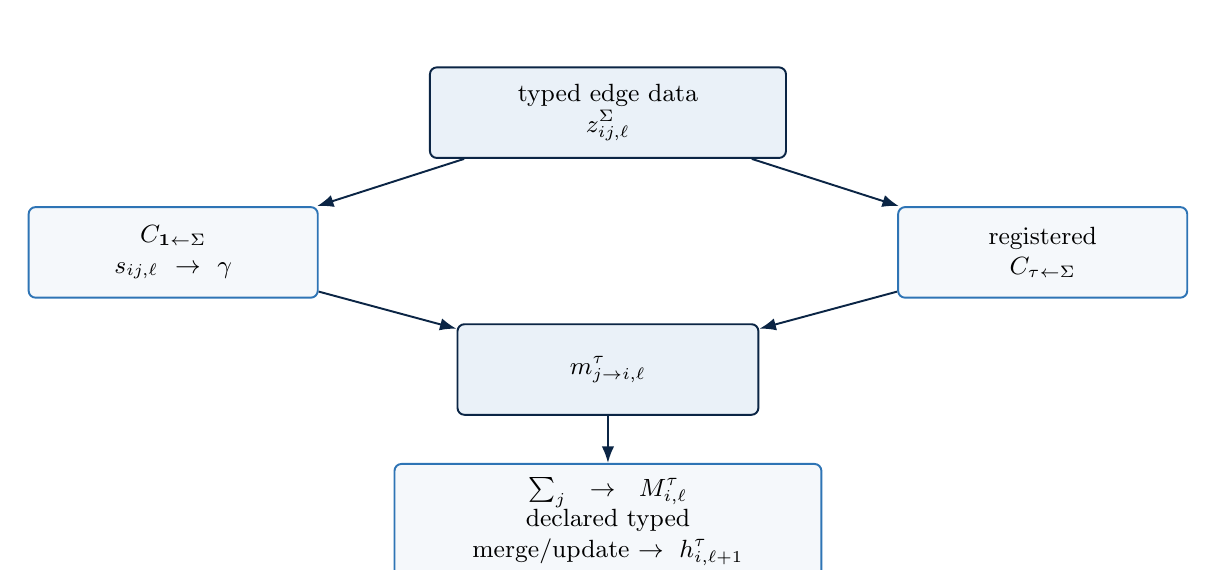
\begin{tikzpicture}[node distance=6mm and 14mm]
  \node[flowStrong,text width=4.1cm] (z) {typed edge data\\$z_{ij,\ell}^{\Sigma}$};
  \node[flow,text width=3.25cm,below left=of z] (inv) {$C_{\one\leftarrow\Sigma}$\\$s_{ij,\ell}\to\gamma$};
  \node[flow,text width=3.25cm,below right=of z] (cov) {registered\\$C_{\tau\leftarrow\Sigma}$};
  \node[flowStrong,text width=3.4cm,below=9mm of $(inv)!0.5!(cov)$] (msg) {$m_{j\to i,\ell}^{\tau}$};
  \node[flow,text width=5.0cm,below=of msg] (upd) {$\sum_j\to M_{i,\ell}^{\tau}$\\declared typed merge/update $\to h_{i,\ell+1}^{\tau}$};
  \draw[arr] (z)--(inv);
  \draw[arr] (z)--(cov);
  \draw[arr] (inv)--(msg);
  \draw[arr] (cov)--(msg);
  \draw[arr] (msg)--(upd);
\end{tikzpicture}
\end{center}

所有消息都在同一 root fiber 中。共享 edge map 与 $\sum_j$ 给出固定根下的非根分子重标号等变；无需边 frame 或相对姿态 transporter。

\subsection{$A\to B$：线性 lift 与非线性 lift}

令 $a\in V_A$，把 B blocks 堆叠为 $\bm b=(b^{(1)},\ldots,b^{(q)})^\top$。线性 lift 只是一列合法 intertwiner blocks 的乘法：
\begin{equation}
  \Delta\bm b_{A\to B}^{\mathrm{lin}}
  =
  \begin{pmatrix}
    \sum_\alpha w_{1\alpha}L_{B^{(1)}\leftarrow A,\alpha}\\
    \vdots\\
    \sum_\alpha w_{q\alpha}L_{B^{(q)}\leftarrow A,\alpha}
  \end{pmatrix}a,
  \qquad
  L_{B^{(r)}\leftarrow A,\alpha}\rho_A(g)
  =\rho_{B^{(r)}}(g)L_{B^{(r)}\leftarrow A,\alpha}.
  \label{eq:linear-a-b}
\end{equation}
若相应 $\Hom_G(V_A,V_{B^{(r)}})$ 为零，该 block 自然不存在。

非线性 pure-A lift 仍由同一个 $C$ 定义：
\begin{equation}
  \Delta b_{A\to B^{(r)}}^{\mathrm{nonlin}}
  =\sum_{p\ge2}\sum_\alpha
  \gamma_{r,p,\alpha}(s)
  \mathcal C_{B^{(r)}\leftarrow (A,p),\alpha}(a),
  \qquad
  C_{B^{(r)}\leftarrow(A,p),\alpha}
  \in\Hom_G(\Sym^pV_A,V_{B^{(r)}}).
  \label{eq:nonlinear-a-b}
\end{equation}
因此 linear lift 与 nonlinear lift 不是两套数学模块：区别仅在 signature 是 $(A,1)$ 还是 $(A,p)$。

\subsection{$B\to B$：线性 block mixing 与非线性 mixing}

线性更新是受 intertwiner 约束的 block matrix，而不是任意矩阵：
\begin{equation}
  \begin{pmatrix}
    \widetilde b^{(1)}\\[-.2em]\vdots\\[-.2em]\widetilde b^{(q)}
  \end{pmatrix}
  =
  \begin{pmatrix}
    \sum_\alpha w^{11}_\alpha L^{11}_\alpha&\cdots&\sum_\alpha w^{1q}_\alpha L^{1q}_\alpha\\
    \vdots&\ddots&\vdots\\
    \sum_\alpha w^{q1}_\alpha L^{q1}_\alpha&\cdots&\sum_\alpha w^{qq}_\alpha L^{qq}_\alpha
  \end{pmatrix}
  \begin{pmatrix}
    b^{(1)}\\[-.2em]\vdots\\[-.2em]b^{(q)}
  \end{pmatrix},
  \quad
  L^{rs}_\alpha\rho_{B^{(s)}}(g)
  =\rho_{B^{(r)}}(g)L^{rs}_\alpha.
  \label{eq:linear-b-b}
\end{equation}
这正是“线性 B$\to$B 通路”；非对角 block 允许在\emph{不同} B spaces 之间混合，只要对应 $\Hom_G$ 非零。

非线性 B mixing 的代表形式为
\begin{align}
  \Delta b^{(r)}_{B/B}
  =&\sum_{s,t,\alpha}
  \gamma_{rst\alpha}(s)
  \mathcal C_{B^{(r)}\leftarrow B^{(s)}B^{(t)},\alpha}
  (b^{(s)},\widetilde b^{(t)})
  \nonumber\\
  &+\sum_{s,p\ge2,\alpha}
  \widetilde\gamma_{rsp\alpha}(s)
  \mathcal C_{B^{(r)}\leftarrow(B^{(s)},p),\alpha}(b^{(s)}).
  \label{eq:nonlinear-b-b}
\end{align}
第一行用于独立 slots，source 是 $V_{B^{(s)}}\otimes V_{B^{(t)}}$；第二行重复同一输入，source 是 $\Sym^pV_{B^{(s)}}$。

\subsection{General molecule 的 $\cA$ 与 $\cB$ 到底包含什么}

先由离线 manifest 给出有限 type set，再由网络需要的 signatures 集合 $\mathfrak S$ 定义
\begin{align}
  \cA(\mathfrak S)
  &:=\bigoplus_{\Sigma\in\mathfrak S}\Hom_G(W_\Sigma,V_A),\\
  \cB(\mathfrak S)
  &:=\bigoplus_{r\in\mathcal R_B}
  \bigoplus_{\Sigma\in\mathfrak S}\Hom_G(W_\Sigma,V_{B^{(r)}}).
  \label{eq:general-banks}
\end{align}
所以 $C_A,C_B$ 不是某几个手写公式，而是按输出类型分区后的完整 typed Hom-space registry。

\begin{center}
\small
\begin{tabularx}{\linewidth}{>{\bfseries\raggedright\arraybackslash}p{.22\linewidth} >{\raggedright\arraybackslash}p{.34\linewidth} X}
\toprule
$\cB$ 子族 & source signature & 作用 \\
\midrule
linear A lift & $V_A\to V_{B^{(r)}}$ & A$\to$B 的 block column\\
linear B mixing & $V_{B^{(s)}}\to V_{B^{(r)}}$ & 对角与跨 B-space block\\
pure-A polynomial & $\Sym^pV_A\to V_{B^{(r)}}$ & 非线性 A$\to$B lift\\
A/B mixed & $\Sym^pV_A\otimes\prod_s\Sym^{q_s}V_{B^{(s)}}\to V_{B^{(r)}}$ & 位置与姿态同边耦合\\
independent B/B & $V_{B^{(s)}}\otimes V_{B^{(t)}}\to V_{B^{(r)}}$ & 跨节点、跨 slot mixing\\
self-B polynomial & $\Sym^pV_{B^{(s)}}\to V_{B^{(r)}}$ & 同一 B feature 的非线性更新\\
\bottomrule
\end{tabularx}
\end{center}
将以上所有 output $B^{(r)}$ 换成 output $A$，便得到 direct-force 所需的 $\cA$。

\subsection{直接 A-head 与世界力}

\begin{align}
  f_i
  &=\sum_{\Sigma,\alpha}
  \gamma_{\Sigma,\alpha}^{\mathrm{out}}(s_{i,L})
  \mathcal C_{A\leftarrow\Sigma,\alpha}(z_{i,L}^{\Sigma}),
  \qquad f_i\mapsto gf_i,
  \label{eq:a-head}\\
  F_i&=O_0f_i.
  \label{eq:world-force}
\end{align}
由于 $g=g_0^\top$ 且 $O_0' = HO_0g^\top$，有
\begin{equation}
  F_i'=HO_0g^\top gf_i=HF_i,
\end{equation}
所以一次 root frame 中得到的 $f_i$ 可由同一固定解码程序变回每个分子的世界坐标受力。

\section{两个说明性分子}

下面两例只说明同一编译器如何实例化；网络与 $C$ 的定义不硬编码任何分子名称。

\subsection{Benzene：$D_6^{\mathrm{rot}}$ 与 $V_2\oplus V_6$}

采用只含 proper rotations 的群
\begin{equation}
  G=D_6^{\mathrm{rot}}
  =\langle r,s\mid r^6=s^2=e,\ srs=r^{-1}\rangle,
  \qquad r=R_z(\pi/3),\quad s=R_x(\pi).
\end{equation}
它不包含镜像、反演或其他 improper operations。令
\begin{equation}
  A=V_1,
  \qquad B^{(1)}=V_2,
  \qquad B^{(2)}=V_6,
\end{equation}
其中 $V_\ell=\STF^\ell(\R^3)$。一组可解释的固定 templates 是
\begin{align}
  \overline B^{(1)}
  &=\STF_2(e_z^{\otimes2})
  =e_ze_z^\top-\tfrac13I_3,\\
  \overline B^{(2)}
  &=\STF_6\!\left(\Re[(e_x+\mathrm i e_y)^{\otimes6}]\right),
\end{align}
并取 $B_i^{(r)}=D^{\ell_r}(R_i)\overline B^{(r)}$。

有限群还允许整个 $\SO(3)$ 不允许的 linear lift。令 $n=e_z$、$Ja=n\times a$，并用 $\odot$ 表示对称张量积，则 benzene 的
$\Hom_{D_6^{\mathrm{rot}}}(A,B^{(1)})$ 唯一方向可显式取为
\begin{equation}
  L_{B^{(1)}\leftarrow A}(a)=\PiSTF{2}\bigl(n\odot Ja\bigr).
  \label{eq:benz-linear-a-b}
\end{equation}
到 $B^{(2)}$ 则有三个独立 linear directions；它们与式\,\eqref{eq:benz-linear-a-b} 一样由 $r,s$ 的生成元方程离线注册。

\subsubsection{显式、平滑的 structured $C$}

令 $a\in A$、$S,T\in B^{(1)}$、$H,K\in B^{(2)}$，$\PiSTF{\ell}$ 表示 rank-$\ell$ STF 投影。pure-A lifts 为
\begin{align}
  \mathcal C_{B^{(1)}\leftarrow(A,2)}(a)
  &=\PiSTF{2}(a^{\otimes2})
  =aa^\top-\tfrac{\|a\|^2}{3}I_3,
  \label{eq:benz-a2}\\
  \mathcal C_{B^{(2)}\leftarrow(A,6)}(a)
  &=\PiSTF{6}(a^{\otimes6}).
  \label{eq:benz-a6}
\end{align}
一个直接 A 型混合及一个高阶力方向为
\begin{align}
  [\mathcal C_{A\leftarrow AB^{(1)}}(a,S)]_u
  &=S_{uv}a_v,
  \label{eq:benz-ca2}\\
  [\mathcal C_{A\leftarrow A^5B^{(2)}}(a,H)]_u
  &=H_{uv_2\cdots v_6}a_{v_2}\cdots a_{v_6}.
  \label{eq:benz-ca6}
\end{align}
例如式\,\eqref{eq:benz-ca2} 在 $a'=ga$、$S'=gSg^\top$ 下满足
$S'a'=gSa$；Jacobian 为 $D_a(Sa)=S$，因此协变性和梯度均是显式的。
独立的 $100$ 次随机 $\SO(3)$ 数值测试给出的最大协变误差为 $9.42\times10^{-16}$。

便宜的 A/B structured maps 包括
\begin{align}
  [\mathcal C_{B^{(1)}\leftarrow AB^{(1)}}(a,S)]_{ij}
  &=\PiSTF{2}\!\left(
  \epsilon_{ik\ell}a_kS_{\ell j}
  +\epsilon_{jk\ell}a_kS_{i\ell}
  \right),\\
  [\mathcal C_{B^{(2)}\leftarrow AB^{(2)}}(a,H)]_{i_1\cdots i_6}
  &=\PiSTF{6}\!\left(
  \sum_{q=1}^{6}\epsilon_{i_qk\ell}a_k
  H_{i_1\cdots i_{q-1}\ell i_{q+1}\cdots i_6}
  \right).
  \label{eq:benz-ab-fast}
\end{align}
便宜的 B/B structured maps 包括
\begin{align}
  \mathcal C_{B^{(1)}\leftarrow B^{(1)}B^{(1)}}(S,T)
  &=\PiSTF{2}(ST+TS),\\
  \mathcal C_{B^{(2)}\leftarrow B^{(1)}B^{(2)}}(S,H)
  &=\PiSTF{6}\!\left(S_{i_1k}H_{ki_2\cdots i_6}\right),\\
  \mathcal C_{B^{(1)}\leftarrow B^{(2)}B^{(2)}}(H,K)
  &=\PiSTF{2}\!\left(H_{ia_1\cdots a_5}K_{ja_1\cdots a_5}\right),\\
  \mathcal C_{B^{(2)}\leftarrow B^{(2)}B^{(2)}}(H,K)
  &=\PiSTF{6}\!\left(H_{i_1i_2i_3abc}K_{i_4i_5i_6abc}\right).
  \label{eq:benz-bb-fast}
\end{align}
这些公式对整个 $\SO(3)$ 协变，因此必然属于合法的 $D_6^{\mathrm{rot}}$ bank；它们只是可解释的 structured 子基，不等于完整 finite-$D_6$ basis。

\subsubsection{完整 benzene $\cB$ 的组成}

直接用 $r,s$ 两个生成元约束求零空间，得到以下完整 finite-$D_6$ 维数；没有群平均。

\begin{center}
\small
\begin{tabular}{lrr}
\toprule
source & $\dim\Hom_G(\cdot,B^{(1)})$ & $\dim\Hom_G(\cdot,B^{(2)})$\\
\midrule
$A$ & 1 & 3\\
$B^{(1)}$ & 3 & 6\\
$B^{(2)}$ & 6 & 15\\
$A\otimes B^{(1)}$ & 6 & 16\\
$A\otimes B^{(2)}$ & 16 & 42\\
$B^{(1)}\otimes B^{(1)}$（独立） & 11 & 28\\
$B^{(1)}\otimes B^{(2)}$（独立） & 28 & 71\\
$B^{(2)}\otimes B^{(2)}$（独立） & 71 & 184\\
$\Sym^2B^{(1)}$（同一输入） & 8 & 18\\
$\Sym^2B^{(2)}$（同一输入） & 42 & 103\\
\bottomrule
\end{tabular}
\end{center}

pure-A lift 在 $p=1,\ldots,6$ 时可压缩写成
\begin{equation}
\left(
\dim\Hom_G(\Sym^pA,B^{(1)}),
\dim\Hom_G(\Sym^pA,B^{(2)})
\right)
=
\begin{cases}
(1,3),&p=1,\\
(4,8),&p=2,\\
(3,10),&p=3,\\
(8,18),&p=4,\\
(7,21),&p=5,\\
(14,33),&p=6.
\end{cases}
\label{eq:benz-pure-a-dims}
\end{equation}
特别地，linear B block 是
\begin{equation}
\binom{\widetilde b^{(1)}}{\widetilde b^{(2)}}
=
\begin{pmatrix}
\sum_{\alpha=1}^{3}w^{11}_\alpha L^{11}_\alpha&
\sum_{\alpha=1}^{6}w^{12}_\alpha L^{12}_\alpha\\
\sum_{\alpha=1}^{6}w^{21}_\alpha L^{21}_\alpha&
\sum_{\alpha=1}^{15}w^{22}_\alpha L^{22}_\alpha
\end{pmatrix}
\binom{b^{(1)}}{b^{(2)}}.
\label{eq:benz-linear-block}
\end{equation}
因此只保留两个 SO(3) 对角 identity 会丢掉有限群允许的跨空间与同空间方向；完整表达由 registry 中全部 $30$ 个 linear B-block directions 给出。
上述维数由独立的 generator-only SVD 核验：覆盖 $34$ 个 signatures，最大零奇异值为
$1.95\times10^{-15}$，最小正奇异值为 $1.00$（判零阈值 $10^{-8}$）。

\subsection{C$_{60}$：proper icosahedral group $I$ 与 $V_6\oplus V_{10}$}

理想 C$_{60}$ 的完整点群是 $I_h$；本项目只取其 proper-rotation subgroup
\begin{equation}
  G=I_h\cap\SO(3)=I\cong A_5,
  \qquad |I|=60.
\end{equation}
一个简洁的 manifest 可选
\begin{equation}
  A=V_1,
  \qquad B^{(1)}=V_6,
  \qquad B^{(2)}=V_{10}.
\end{equation}
若 $q_a\in\R^3$ 是 body frame 中的 $60$ 个碳原子坐标，可取原子云 STF moments
\begin{equation}
  \overline B_\ell
  =\PiSTF{\ell}\!\left(\sum_{a=1}^{60}q_a^{\otimes\ell}\right),
  \qquad \ell\in\{6,10\}.
  \label{eq:c60-atom-anchor}
\end{equation}
这里求和对象是原子，不是群元素，所以式\,\eqref{eq:c60-atom-anchor} 不是群平均。等价地，可从 $I=\langle u,v\mid u^5=v^3=(uv)^2=e\rangle$ 的两个输入生成元直接编译固定子空间：
\begin{equation}
  (D^\ell(u)-I)\overline B_\ell=0,
  \qquad
  (D^\ell(v)-I)\overline B_\ell=0.
\end{equation}
pose descriptors 为
\begin{equation}
  B_i^{(1)}=D^6(R_i)\overline B_6,
  \qquad
  B_i^{(2)}=D^{10}(R_i)\overline B_{10},
\end{equation}
并再次满足 $B_i^{(r)}(gR_i g_i)=D^{\ell_r}(g)B_i^{(r)}(R_i)$，故 $g_i$ 消失。

\subsubsection{C$_{60}$ 的 linear 与 nonlinear $C_B$ 例子}

proper-$I$ 下两个 linear lift 均存在，且各有一个独立方向：
\begin{equation}
  \dim\Hom_I(V_1,V_6)=1,
  \qquad
  \dim\Hom_I(V_1,V_{10})=1.
\end{equation}
一个无需 irrep 表的显式构造是
\begin{equation}
  L_{\ell\leftarrow1}(a)=J_\ell(a)\overline B_\ell,
  \qquad \ell\in\{6,10\},
  \label{eq:c60-linear}
\end{equation}
其中 $J_\ell(a)$ 是 rank-$\ell$ STF 表示中绕向量 $a$ 的无穷小旋转生成矩阵。由于
$D^\ell(g)J_\ell(a)D^\ell(g)^{-1}=J_\ell(ga)$ 且 $D^\ell(g)\overline B_\ell=\overline B_\ell$，式\,\eqref{eq:c60-linear} 满足 intertwiner law。

一组处处多项式可微的 nonlinear structured maps 是
\begin{align}
  \mathcal C_{B^{(1)}\leftarrow(A,6)}(a)
  &=\PiSTF{6}(a^{\otimes6}),\\
  \mathcal C_{B^{(2)}\leftarrow(A,10)}(a)
  &=\PiSTF{10}(a^{\otimes10}),\\
  \mathcal C_{B^{(2)}\leftarrow A^4B^{(1)}}(a,H_6)
  &=\PiSTF{10}\Sym(a^{\otimes4}\otimes H_6),\\
  [\mathcal C_{B^{(2)}\leftarrow B^{(1)}B^{(1)}}(H_6,K_6)]_{i_1\cdots i_{10}}
  &=\PiSTF{10}\Sym\!\left(
  H_{i_1\cdots i_5p}K_{i_6\cdots i_{10}p}
  \right),\\
  [\mathcal C_{A\leftarrow A^5B^{(1)}}(a,H_6)]_i
  &=H_{ij_1\cdots j_5}a_{j_1}\cdots a_{j_5}.
  \label{eq:c60-maps}
\end{align}
这些是对整个 $\SO(3)$ 都成立的 structured fast paths，因而必然属于 finite-$I$ bank；完整 $I$-only $\cA/\cB$ 仍由式\,\eqref{eq:null-basis} 的全部零空间给出，不为 C$_{60}$ 编写专用网络层。
上式两个 rank-$6$ tensors 若来自独立节点，则 source 为 $V_6\otimes V_6$；若二者是同一 live tensor，则注册为 $\Sym^2V_6$。

\section{基础数学模块：现有设计}

\begin{center}
\small
\begin{tabularx}{\linewidth}{>{\ttfamily\raggedright\arraybackslash}p{.34\linewidth}X}
\toprule
模块 & 固定职责 \\
\midrule
stf\_space.py / stf\_rep.py
& STF coordinates、representation actions、symmetric powers 与 structured tensor coupling。\\
anchor\_compiler.py
& 从输入 proper-rotation generators 编译固定 anchor spaces；不做群平均。\\
pose\_encoding.py
& 用一次 root-relative $R_i$ 产生分块 $B_i^{(r)}$，并验证右侧 gauge 消失。\\
\_compiler\_utils.py
& CPU float64 nullspace/SVD 与数值诊断后端。\\
intertwiner\_compiler.py
& 建立 source/target generator actions 并求解 $CS_q=T_qC$。\\
covariant\_registry.py
& \texttt{GeneratorSystem}、\texttt{BBlockManifest}、\texttt{TypeCatalog}、\texttt{CSlot/CSignature}、normalized $\Sym^p$、full artifact、basis view、registry 与 runtime。\\
covariants.py
& 解析型 scalar contraction、vector covariant 与 STF structured fast paths。\\
\bottomrule
\end{tabularx}
\end{center}

当前接口的数学契约是：完整 basis、lift 与 view 作为冻结 buffers；forward 不编译；
\texttt{evaluate\_basis} 返回显式 basis outputs，
\texttt{apply\_coefficients} 直接融合完整 basis coefficients，
\texttt{evaluate\_view} 调用显式 basis view；live inputs 和 learned coefficients 保留 autograd。

\section{设计要点：必须守住的灵魂}

\begin{enumerate}
  \item 分子群在本设计中是 $G\subset\SO(3)$ 的 proper-rotation group；例如 $D_6^{\mathrm{rot}}$ 不包含镜像或反演。
  \item 构架面向一般同种刚性分子；benzene 与 C$_{60}$ 只是两个 manifest/diagnostic examples。
  \item 整片分子云只建立一次 root local frame；绝不建立 node-local 或 edge-local frame。
  \item $R_i\to B_i^{(r)}$ 后 sender gauge $g_i$ 永久消失；后续只保留共同 root action $g$。
  \item 任意 $h_{i,\ell}^{\tau}$ 与 $h_{j,k}^{\tau}$ 同型协变，因为它们位于同一 root fiber；跨节点 mixing 不需 transporter。
  \item 若启用 GNN extension，同边 A/B 数据必须先通过 typed $C$ 耦合，再做邻居聚合；否则会丢失“哪个位置对应哪个姿态”。
  \item $C$ 是训练前冻结的完整 typed $\Hom_G$ basis，不是可训练表示、第三条通路或手写的某一个公式。
  \item linear A$\to$B、nonlinear A$\to$B、linear B$\to$B 与 nonlinear B/B 全部是不同 signatures 下的同一个 $C$ 机制。
  \item 不同 B spaces 可以线性混合；存在性与方向数只由对应 $\Hom_G(V_{B^{(s)}},V_{B^{(r)}})$ 决定。
  \item 独立同型 inputs 使用完整 tensor product；只有重复同一 live input 时才使用 normalized $\Sym^p$。
  \item 不变量统一记为 $s$，并由 $C_{\one\leftarrow\Sigma}$ 产生；所有 gates 必须只依赖这些 scalars。
  \item TFENN 协变层禁止 group convolution 与群平均。输入生成元只用于离线方程 $CS_q=T_qC$，不进入网络运行时；明确标注的外部 MLP baseline 可单独使用群平均。
  \item 不预存 irrep 或 CG tables；type partition、anchors 与 $C$ basis 都从输入 generator actions 离线产生。
  \item full basis 永久保存；任何省略或低维 view 都必须显式记录 $P$ 与 rank，完整表达的含义不可被静默改变。
  \item 固定 $C$ 的 polynomial contraction 与 smooth gates 保证梯度存在；离线 nullspace/SVD 不参与反向传播。
  \item 每个模型必须显式声明 covariant flow、raw covariant access、invariant context、A/B path families、same-type bypass、channel mixing 与 Gate contract。
  \item 若启用 GNN extension，共享 edge program 与对邻居求和保证固定根下的分子重标号等变；根的选择是一次性结构约定。
  \item 世界力只由 $F_i=O_0f_i$ 解码。直接 A-head 保证协变，但“直接力”本身不等价于自动满足保守力条件。
\end{enumerate}

\begin{designbox}
\textbf{最终设计判据。}
未来任何实现都应能逐项证明：一次 root frame、B 消右 gauge、所有 hidden tensors 共用 root action、typed $C$ 完整基、不变量门控、声明明确的 typed flow 与 mixing contract、直接 A-head，以及 $F_i=O_0f_i$ 的世界坐标解码；若使用 GNN，还必须证明 permutation-symmetric aggregation。
\end{designbox}

\end{document}
